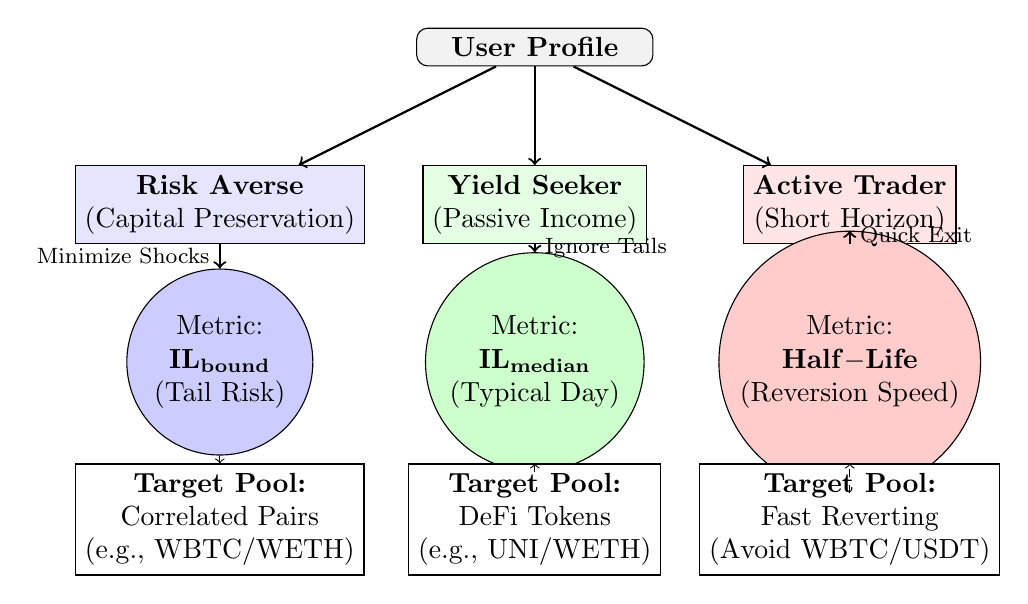
\begin{tikzpicture}[node distance=2cm, auto]
        % Nodes
        \node (user) [draw, rectangle, rounded corners, fill=gray!10, minimum width=3cm, align=center] {\textbf{User Profile}};
        
        \node (risk_averse) [draw, rectangle, below of=user, xshift=-4cm, fill=blue!10, minimum width=2.5cm, align=center] {\textbf{Risk Averse}\\(Capital Preservation)};
        \node (yield) [draw, rectangle, below of=user, fill=green!10, minimum width=2.5cm, align=center] {\textbf{Yield Seeker}\\(Passive Income)};
        \node (active) [draw, rectangle, below of=user, xshift=4cm, fill=red!10, minimum width=2.5cm, align=center] {\textbf{Active Trader}\\(Short Horizon)};

        \node (metric1) [draw, circle, below of=risk_averse, fill=blue!20, align=center] {Metric:\\$\mathbf{IL_{bound}}$\\(Tail Risk)};
        \node (metric2) [draw, circle, below of=yield, fill=green!20, align=center] {Metric:\\$\mathbf{IL_{median}}$\\(Typical Day)};
        \node (metric3) [draw, circle, below of=active, fill=red!20, align=center] {Metric:\\$\mathbf{Half\text{-}Life}$\\(Reversion Speed)};

        \node (pool1) [draw, rectangle, below of=metric1, fill=white, align=center] {\textbf{Target Pool:}\\Correlated Pairs\\(e.g., WBTC/WETH)};
        \node (pool2) [draw, rectangle, below of=metric2, fill=white, align=center] {\textbf{Target Pool:}\\DeFi Tokens\\(e.g., UNI/WETH)};
        \node (pool3) [draw, rectangle, below of=metric3, fill=white, align=center] {\textbf{Target Pool:}\\Fast Reverting\\(Avoid WBTC/USDT)};

        % Edges
        \draw[->, thick] (user) -- (risk_averse);
        \draw[->, thick] (user) -- (yield);
        \draw[->, thick] (user) -- (active);

        \draw[->, thick] (risk_averse) -- node[left, font=\footnotesize] {Minimize Shocks} (metric1);
        \draw[->, thick] (yield) -- node[right, font=\footnotesize] {Ignore Tails} (metric2);
        \draw[->, thick] (active) -- node[right, font=\footnotesize] {Quick Exit} (metric3);

        \draw[->, dashed] (metric1) -- (pool1);
        \draw[->, dashed] (metric2) -- (pool2);
        \draw[->, dashed] (metric3) -- (pool3);
        
    \end{tikzpicture}